
\subsection{Endpoint prediction}

Task B is formulated as multi-label node classification on a heterogeneous, per-patient graph. 
Rather than building one global graph and treating patients as additional nodes, every patient is represented 
as a copy of the same fixed causal DAG topology, with node feature vectors instantiated from that patient's 
individual covariates. The prediction targets are a fixed subset of clinical events on patient site. 
Formally, for a patient graph \(G_p = (V, E)\) shared across the cohort, with patient-specific node features
\(x_p\), the model computes

\[
\hat{y}_{p,e} = \sigma\big(f_\theta(G_p, x_p)_e\big), \quad e \in \mathcal{E}_{\text{target}}
\]

where \(f_\theta\) is a heterogeneous graph neural network shared across all patients, and only the leaf-level
target embeddings are read out by the classification head.

\subsubsection{Data Representation}

The first thing in applying GNNs is to built properly the input into neural network. The input graph for the node 
classification task was built based on: 

\begin{enumerate}[label=\alph*)]
    \item \textbf{nodes}
    \item \textbf{edges}
    \item \textbf{per-scenario patient sample table} 
\end{enumerate}

Based on those items \texttt{HeteroData} object was created which was represented by objects type presented in the table

\begin{table}[t]
    \centering
    \caption{Components of the per-patient \texttt{HeteroData} graph representation.}
    \label{tab:heterodata_components}
    \begin{tabularx}{\textwidth}{@{}l X@{}}
        \toprule
        \textbf{Component} & \textbf{Description} \\
        \midrule
        Node types &
        Six semantic categories of nodes shared across all patient graphs: \texttt{patient\_context}, \texttt{drug\_exposure}, \texttt{mechanism}, \texttt{adr\_or\_intermediate\_state}, \texttt{observation\_or\_selection}, and \texttt{clinical\_endpoint}. \\
        \addlinespace
        Relations &
        Keyed by \texttt{(src\_type, "to", dst\_type)} weighted by \texttt{edge\_attr} instead of using \texttt{edge\_type}. This keeps the number of distinct convolutional relation modules in \texttt{HeteroConv} small while still letting edge-type information reach the message function. \\
        \addlinespace
        Edge attributes (\texttt{edge\_attr}) &
        %signed effect size, activation frequency, mechanistic confidence, evidence weight, and the edge-type one-hot. Convolutions consuming a scalar \texttt{edge\_weight} (GraphConv/GCN) receive only the signed effect-size column; convolutions consuming a full \texttt{edge\_attr} (GAT, Transformer) receive the whole vector. \\
        Combination of \texttt{effect\_size} and \texttt{effect\_sign} \\
        \addlinespace
        Node features (\texttt{x}) &
        The patient's observed values for that node where the node. \\
        \bottomrule
    \end{tabularx}
\end{table}

The patient data is encoded on nodes level. In \cref{fig:architecture} there is presented the exemplary DAG for one 
of patient. 

\begin{figure}[h]
    \centering
    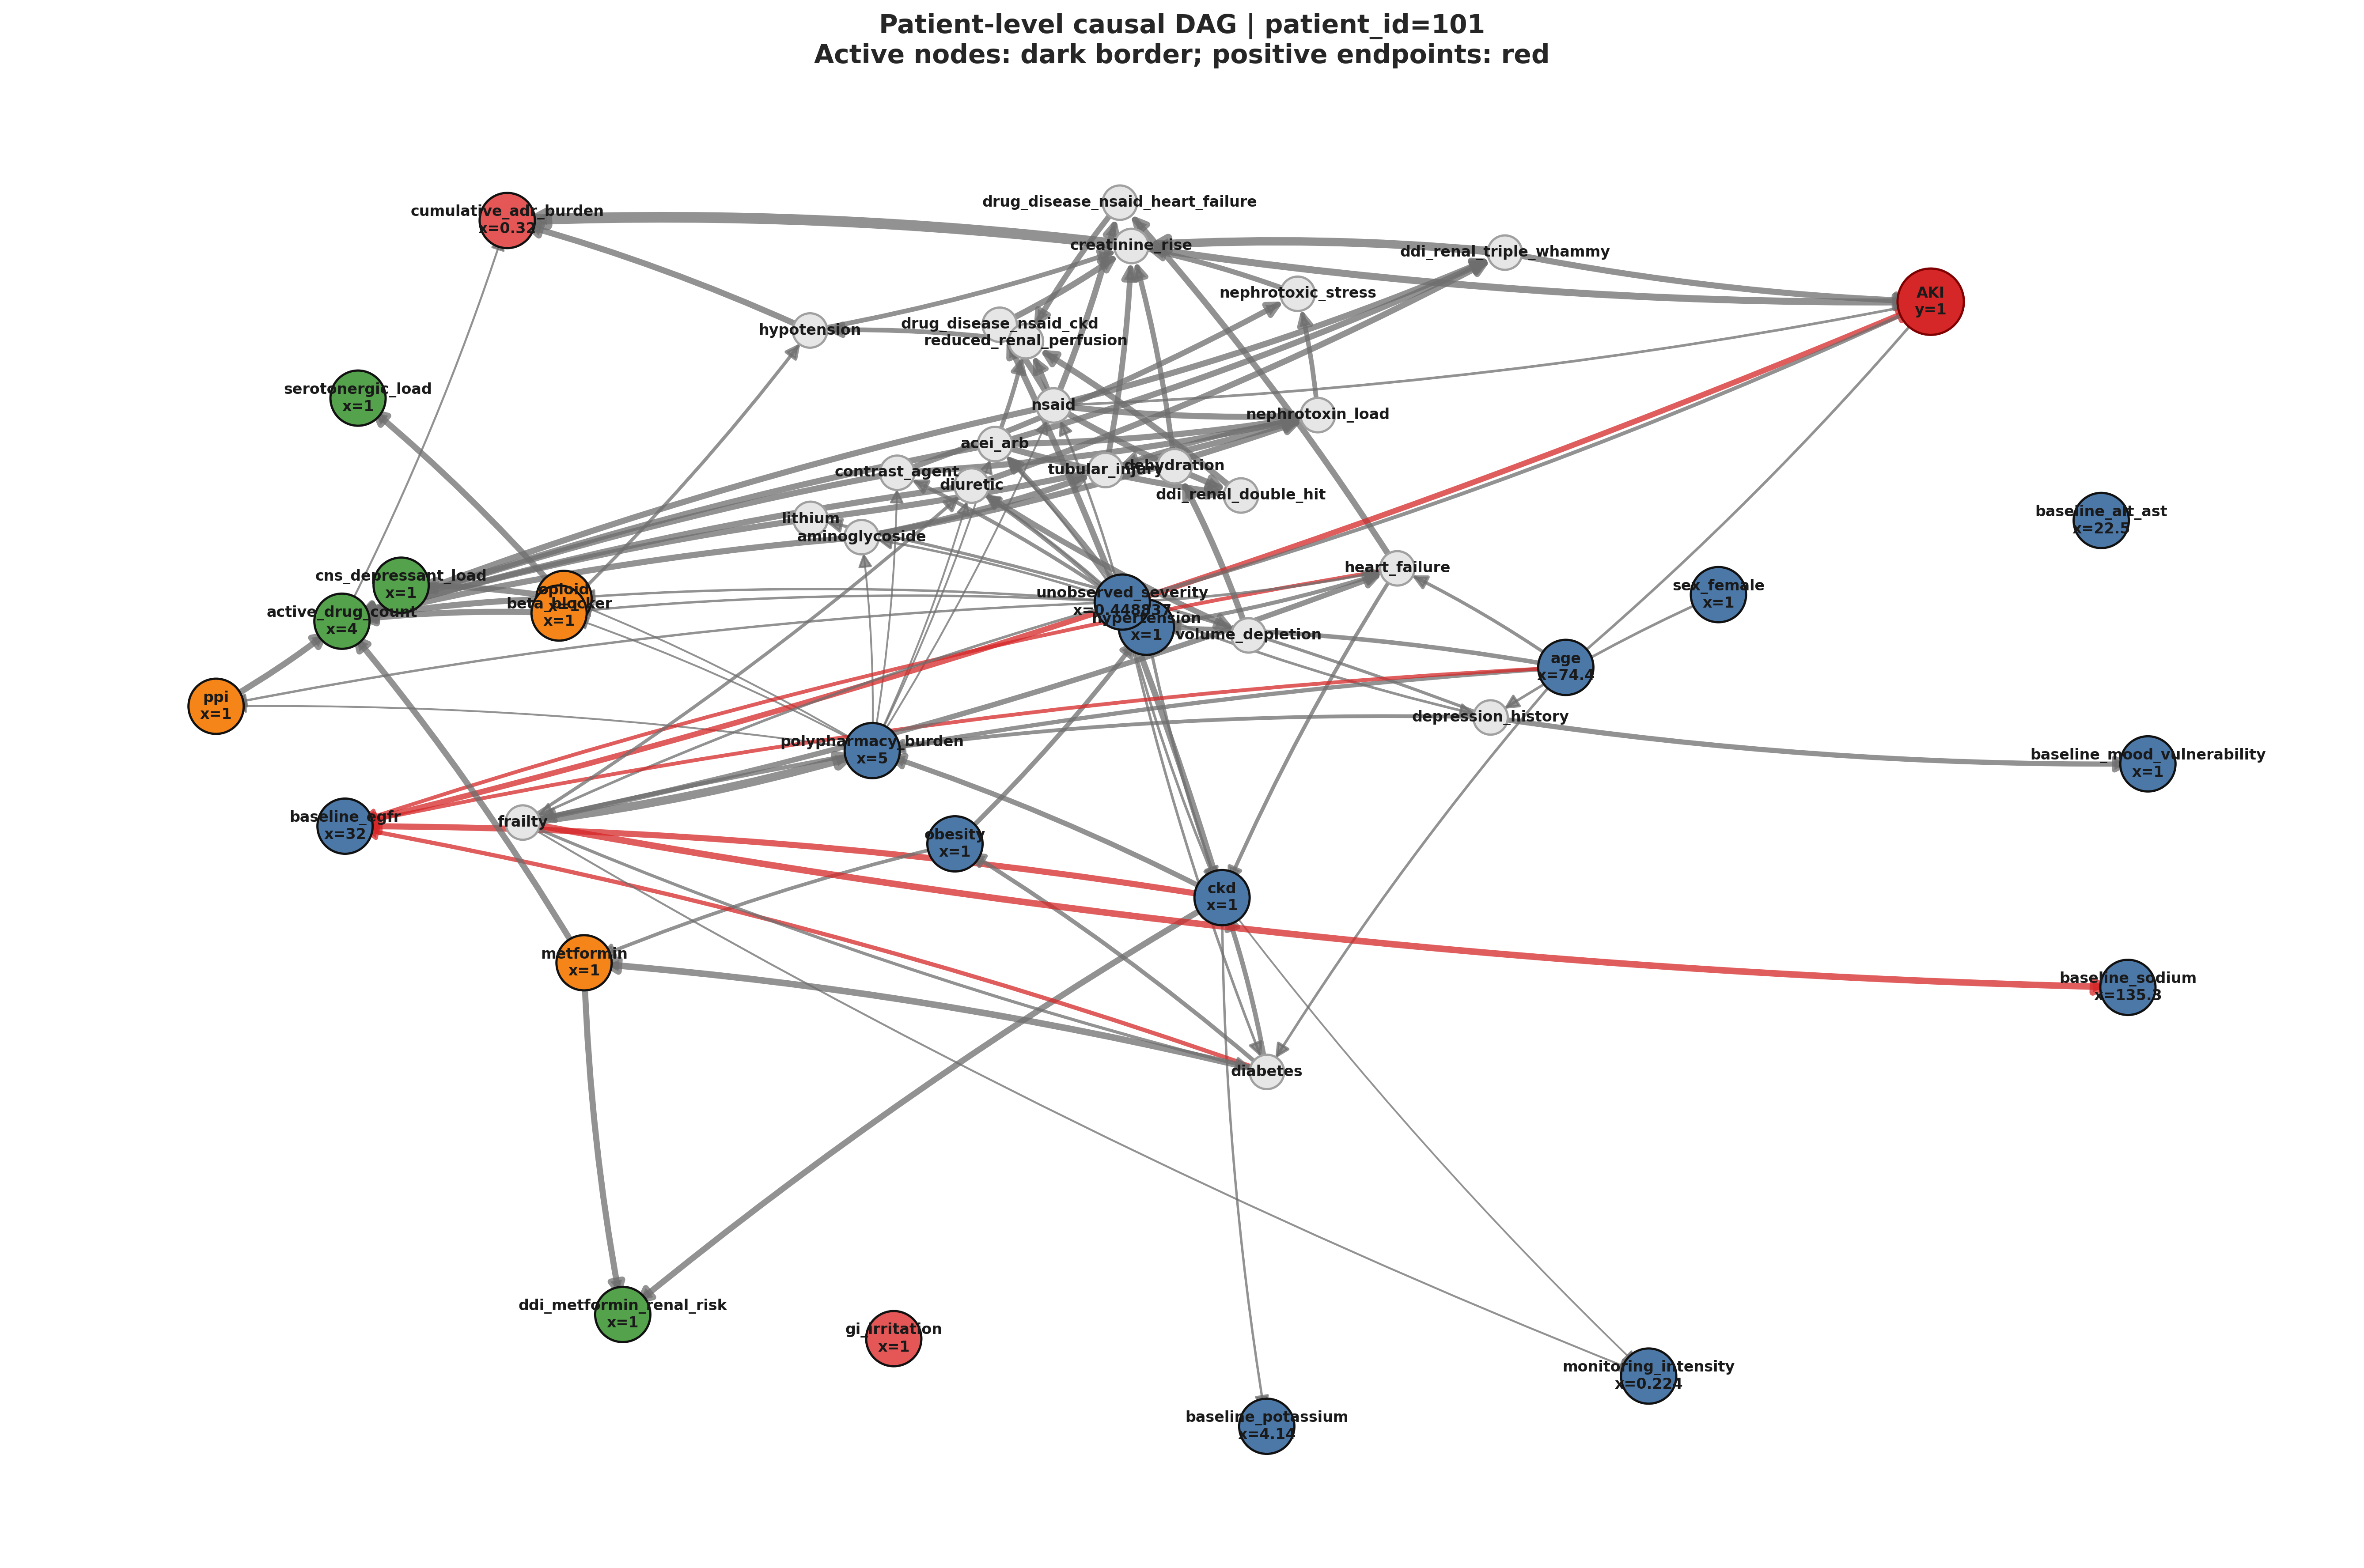
\includegraphics[width=\textwidth, height=0.45\textheight, keepaspectratio]{rysunki/patient_dag_101.png}
    \caption{The description of the two tasks addressed in the thesis.}
    \label{fig:patient_dag}
\end{figure}

Two structural exclusion mechanisms are applied before any feature is computed: 
\begin{enumerate}[label=\alph*)]
    \item nodes flagged \texttt{exclude\_from\_observed\_model} or \texttt{is\_latent} (hidden confounders); 
    \item nodes that are structural descendants of any endpoint in the DAG (e.g. documentation nodes such as 
    \texttt{hospital\_contact}, \texttt{fall\_reported}, which are caused by the endpoint rather than causal parents of it)
\end{enumerate}

 All normalization statistics (mean/std for continuous node values) 
 and all HCR evidence statistics (\cref{subsec:hcr_application}) are computed exclusively on the training split of patients, to 
 prevent both node-level and patient-level information leakage across splits.
 %trzeba dopisać wybor endpoints - dlaczego tak a nie inaczej
 %auc liczony bez endpoint Serotonin_syndrome Rhabdomyolysis Lactic_acidosis - bardzo rzadkich 

\subsubsection{Model architecture}

The core architecture is a stack of heterogeneous graph convolutional layers wrapped in \texttt{HeteroConv},
shared across relation types but parameterized identically for every patient graph. Four convolution backbones 
are supported through a common registry and were benchmarked against each other: GraphSAGE, and TransformerConv. 
As these operators were originally designed for homogeneous graphs,
each is instantiated once per edge type inside \texttt{HeteroConv}, so the heterogeneous DAG is handled without 
collapsing node/edge types into a single homogeneous graph.
As benefit of casual graph structure is possibility to encode deep structured path for node classification, 
multiple number of layers was tested to choose the best model.  
%root_weight

A design issue that was handled during experiments is the duplication of the self-transform across relations. 
Several PyG convolution layers (SAGEConv, TransformerConv) internally add their own linear self-loop term,
 wrapped per-relation inside \texttt{HeteroConv}, this term is silently duplicated once per incoming 
relation type for a given node type. The implementation removes this internal duplication 
(\texttt{root\_weight}=False for SAGE/Transformer) and replaces it with a single, explicit, 
controlled self-transform per layer per node type. 
% For GAT-family layers, where the self-dependency is baked into the attention query and cannot be disabled, the explicit self-transform 
% acts as an additional controlled term on top of the irreducible built-in dependency. GraphConv/GCN, which has no 
% \texttt{root\_weight} parameter at all, is deliberately excluded from this mechanism, since its built-in self-transform 
% cannot be removed without reimplementing the layer.
%node identity 

A node-identity embedding, added after the input projection, was introduced to resolve a specific representational 
collapse. Message-passing GNNs are bounded in expressive power by the 1-dimensional Weisfeiler-Lehman graph 
isomorphism test. In the dataset, several 
endpoint nodes of the same type (e.g. Serotonin syndrome, Rhabdomyolysis, Lactic acidosis) share 
identical static audited attributes (e.g. \texttt{severity\_weight}, observability) and comparable topological 
positions, and were therefore indistinguishable to the model except through such positional cues.
To break this symmetry, a learnable embedding table is maintained per node type, indexed by each node's fixed 
local index, and added to the projected input features before the first convolutional layer, following the same 
principle underlying position aware node embeddings in .
%oversmoothing (i will see if i should present it or rephrase it somehow)

This connects directly to the model's handling of oversmoothing. Using multiple message-passing layers risks oversmoothing 
the embedding signal, where repeated aggregation causes node representations to converge toward 
indistinguishability. To mitigate this, several oversmoothing countermeasures were applied: 
residual connections, Jumping Knowledge, DropEdge, and PairNorm. These methods were evaluated both 
individually and in combination with the HCR enrichment described in \cref{subsec:hcr_application}.

\subsubsection{HCR application}
\label{subsec:hcr_application}

In addition to the purely structural GNN pathway, approch presented in the thesis incorporates a statistical evidence 
side-channel - HCR described in details in \cref{subsec:hcr_def}. This channel is motivated by the 
observation that some parent-endpoint dependencies are well captured by simple, well-understood pairwise 
statistics computed directly from the training cohort, and that combining such statistics with the deep GNN 
representation captures the strong signal from direct parents and smoothed signal from further layers.
There were run couple of experiments with HCR configurations and GNNs. However, in general the approach was about
computation of contingency-table statistics for each target endpoint and direct parents or pre-direct parents in 
the audited DAG (restricted to nodes with inferred 
binary, count, or continuous value types). The statistics computed was as followed per (parent, endpoint) 
pair: the \(\varphi\)-coefficient, normalized mutual information, a tanh-scaled log odds 
ratio, risk difference, and a tanh-scaled log lift, plus prevalence and support terms. There are nine to forty-one 
channels depending on configuration.
%dopisac dlaczego u nas jest 41/42 a w przypadku task a 41
%leave-one-out

As these coefficients are computed with the patient's own endpoint label as part of the statistic, a naive 
computation would leak the label into the feature. This was addressed with an 
exact leave-one-out correction: every training patient's coefficient is computed from all other training patients
only, using a closed-form re-weighting of the population statistic.
 
 Continuous and count-valued parents are mapped to comparable pseudo-uniform scores via a train-only empirical 
 CDF transform (with deterministic, patient-ID-seeded jitter for count variables), and Legendre polynomial bases 
 are used to capture non-linear dependence on continuous parents.

 Three integration modes were supported: 
 \begin{enumerate}[label=\alph*)]
    \item linear approach - a single scalar HCR score added directly to the GNN logit,
    \item nonlinear encoder - parent-endpoint evidence vectors pooled and passed through a shared MLP
    \item separate encoders per parent node type - every direct parent passed through a separated MLP
    \item triple relations - relations not only focused on direct parents, but direct parents and grandparents. 
 \end{enumerate}


 The pooling in HCRPairEncoder masks out padding positions (endpoints with fewer parents than the batch's 
 maximum) and returns a neutral zero vector for endpoints with no eligible parents, avoiding division by zero.

%jak jest wszystko polaczone dokladniej


\subsubsection{Training setup}

Training iterates over patient graphs batched via PyG DataLoader. The experiments were run with
targeted binary cross-entropy and focal loss with class-balance-aware weighting. 
Weight and focal alpha were computed from the training split's endpoint prevalence, since clinical outcomes
are rare and highly imbalanced. Model selection uses ReduceLROnPlateau on validation performance, and 
evaluation is reported separately per endpoint and in aggregate, using AUROC, AUPRC, and prevalence-normalized 
lift.
%alongside the representation-level over-smoothing diagnostics (MAD, cosine similarity, Dirichlet energy) 
%used to relate architectural choices. 
 As the synthetic dataset generated for this project contains
 rare events and class imbalance, AUPRC was chosen as a key performance
 metric. It focuses on the positive class and reflects the trade-off
 between precision and recall. Below there are included the equations for calculating metrics.
 
 \emph{AUC} is the area under the receiver operating characteristic curve (ROC-AUC) 
 and is defined as:
 \begin{equation}
   \mathrm{ROC\mbox{-}AUC}
   =
   \int_0^1 \mathrm{TPR}(\mathrm{FPR})\,d\mathrm{FPR}.
   \end{equation}
   where $\mathrm{TPR}$ is the true positive rate and $\mathrm{FPR}$ is the false positive rate.
 
 \emph{AUPRC} is the area under the precision--recall curve and is defined as:
 \begin{equation}
   \mathrm{AP} =
   \sum_{n}
   \left(R_n - R_{n-1}\right) P_n,
   \end{equation}
   where $P_n$ and $R_n$ denote precision and recall at the $n$-th threshold,
   respectively.
 
 \emph{Lift} is the AUPRC divided by the prevalence baseline, that is, the
 factor by which the model improves over a random ranking, e.g. at a mean
 prevalence of $5.5\%$ a lift of $2.3$ corresponds to an AUPRC of $0.125$.
 
 In addition to the traditional metrics described above, an oracle AUC was
 calculated for the node-classification task.
 As the dataset for this task is synthetic,
 the exact function used to generate each endpoint is known, which allows to calculate AUC oracle.
 In the final assesement of the models we compared the AUC and AUC oracle 
 (\%ceiling) with the following formula:
 
 \begin{equation}
   \frac{\mathrm{AUC} - 0.5}{\mathrm{AUC}_{\mathrm{Oracle}} - 0.5} \cdot 100\%,
   \label{eq:pct-ceiling}
 \end{equation}
 %
 where $\mathrm{AUC}_{\mathrm{Oracle}} = 0.651$ is the AUC oracle averaged
 over the same eight endpoints. This metric expresses the
 share of attainable signal recovered by the model. The model increased performance
 is calculated from random baseline model performance which is 0.5.
 
 
 